\chapter{Organizacion}

\begin{figure}[H]
	\centering
	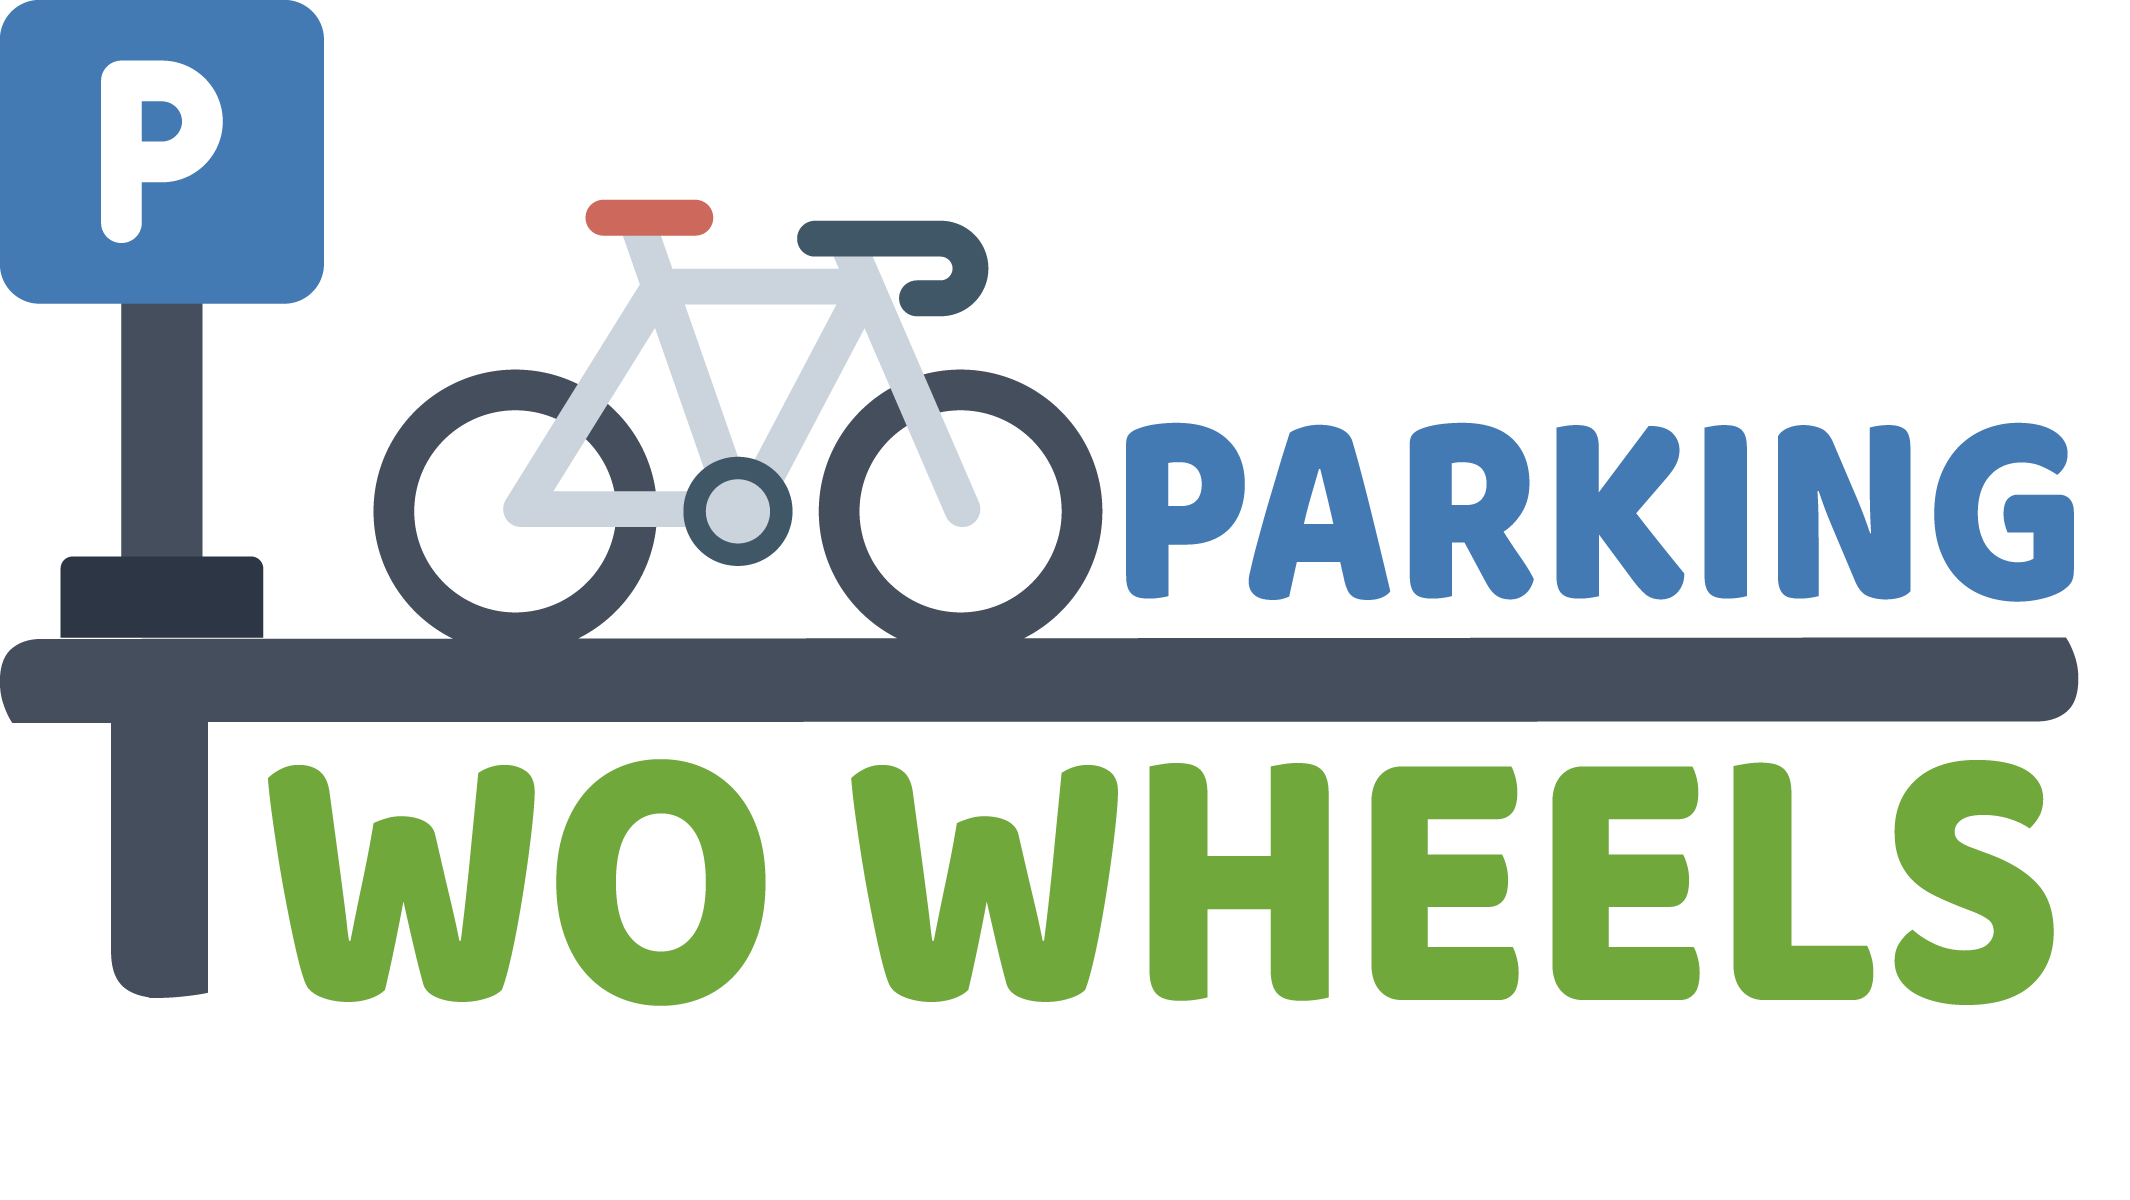
\includegraphics[scale=0.5]{imagenes/logoTWP}
	\caption{Two Wheels Parking}
	\label{fig:logotwp}
\end{figure}


\section{Misión}
En Two Wheels Parking ofrecemos soluciones de aparcamiento para bicicletas en la ciudad de Bogotá, ofreciendo una experiencia de tranquilidad, seguridad y organización a nuestros clientes,  buscando incentivar el uso de este medio de transporte como una alternativa limpia y segura.\\

\section{Visión}
Queremos estar comprometidos con los problemas de nuestros clientes de forma transparente y eficaz, convirtiéndonos en un socio de confianza. En Two Wheels Parking queremos ser un referente como una empresa líder en soluciones de aparcamiento, dando a conocer nuestra marca como una empresa ética, responsable y solidaria con nuestros clientes.\\

\section{Estructura Organizacional}
\begin{figure}[H]
	\centering
	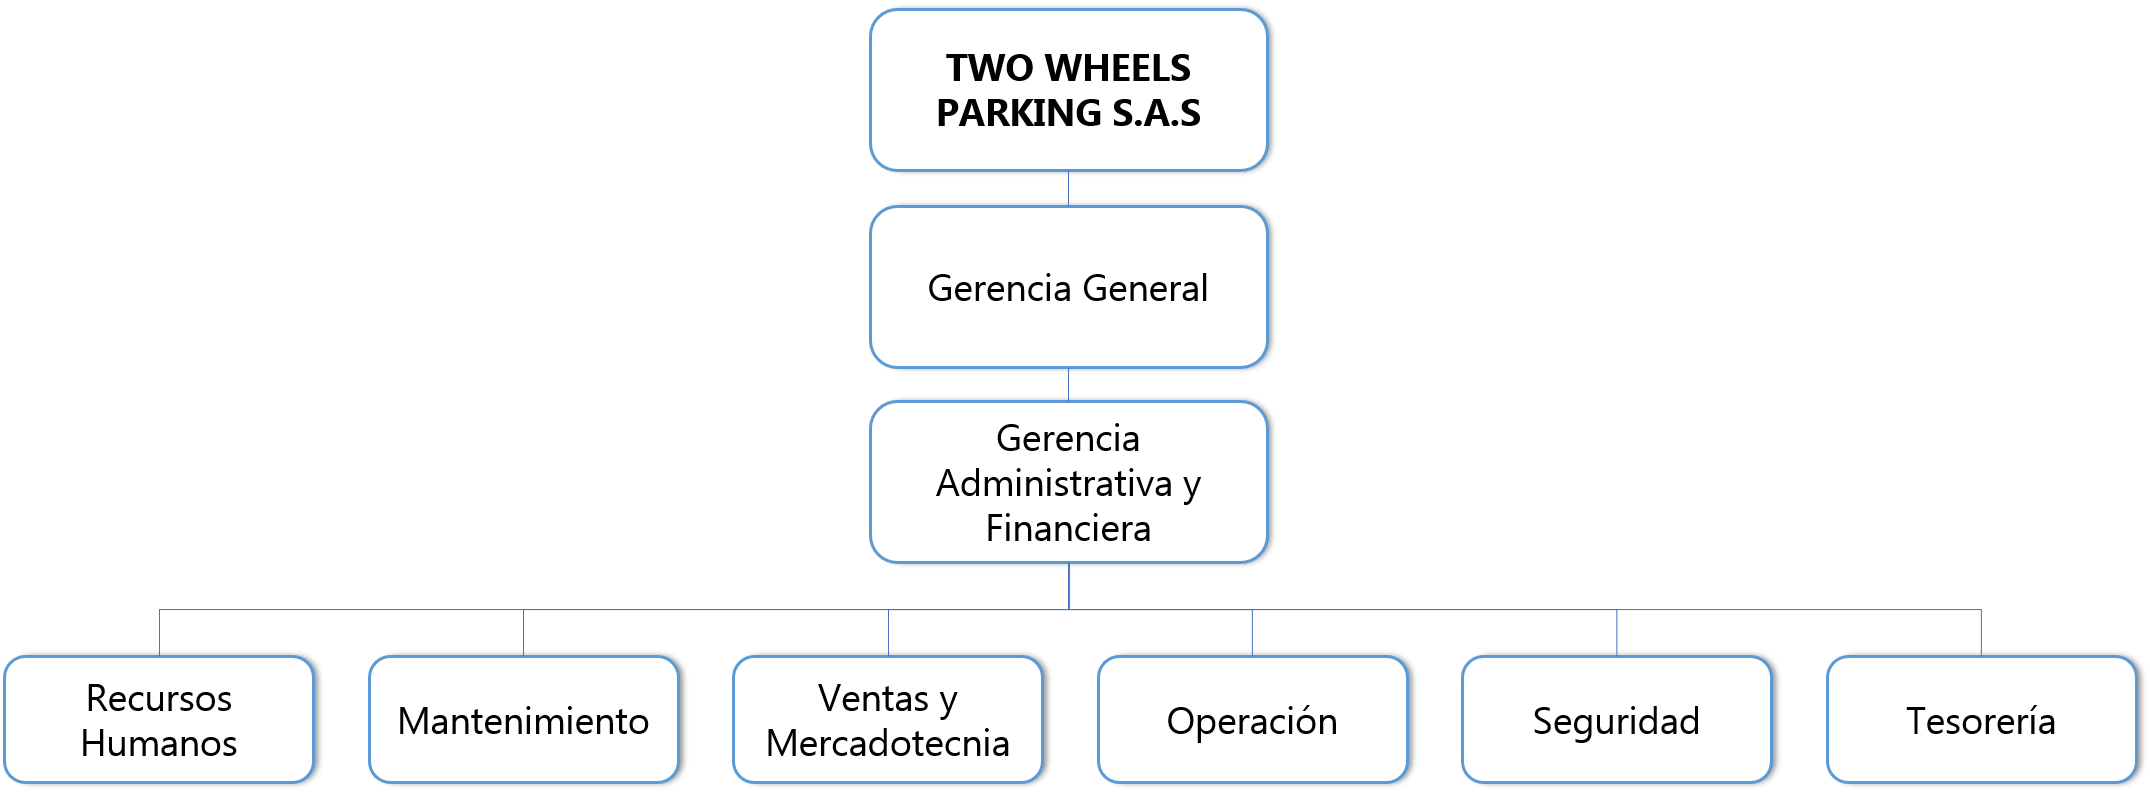
\includegraphics[width=0.7\linewidth]{imagenes/organigrama}
	\caption{Organigrama General de Two Wheels Paking.}
	\label{fig:organigrama}
\end{figure}

\section{Funciones de Negocio y Manual de funciones}

\subsubsection {Recursos humanos}
\begin{itemize}
	\item Trabajadora social: Profesional encargado del desarrollo de vínculos humanos saludables y buenas relaciones sociales entre los individuos que laboran al interior de la empresa.\\
\end{itemize}

\subsubsection {Gerencia}
\begin{itemize}
	\item Presidente: Representante, líder y supervisor en la toma de decisiones que guían el rumbo de la compañía. \\
	\item Secretaria: Principal colaboradora del presidente en el área administrativa, dentro de su rol es la encargada de la gestión de la documentación empresarial y de la atención al público.\\
\end{itemize}

\subsubsection{Seguridad} 
\begin{itemize}
	\item Guardia de seguridad: personal competente para realizar  actividades  de  vigilancia,  inspección,  prevención  y  detección  de  anormalidades  al interior de la Institución.
\end{itemize}

\subsubsection{Tesorería} 
\begin{itemize}
	\item Tesorero: Encargado de gestionar y dirigir los asuntos relacionados con movimientos económicos o flujos monetarios, tanto captación como desembolsos dentro de la empresa.
\end{itemize}

\subsubsection{Administrativo y contable} 
\begin{itemize}
	\item Contador Público: Profesional encargado de realizar y verificar los registros contables, tributarios y financieros de la empresa, generando los informes y documentos legales exigidos por la legislación nacional.
	\item Administrador: Responsable de la gestión de recursos materiales y financieros dedicados a la realización y control de las distintas actividades tanto técnica como administrativas mediante una correcta planificación, coordinación y ejecución.
\end{itemize}

\subsubsection{Ventas y mercadotecnia}
\begin{itemize}
	\item Agentes de ventas: Profesionales capaces de captar y aumentar el número y la calidad de clientes a los cuales la empresa busca prestar una serie de soluciones.
	\item Publicista: Experto en supervisar, coordinar y ejecutar estrategias de publicidad y posicionamiento de imagen tanto de la empresa como de los productos que se generan al interior de ella.
\end{itemize}


\section{Procesos de Negocio}
\begin{figure}[H]
	\centering
	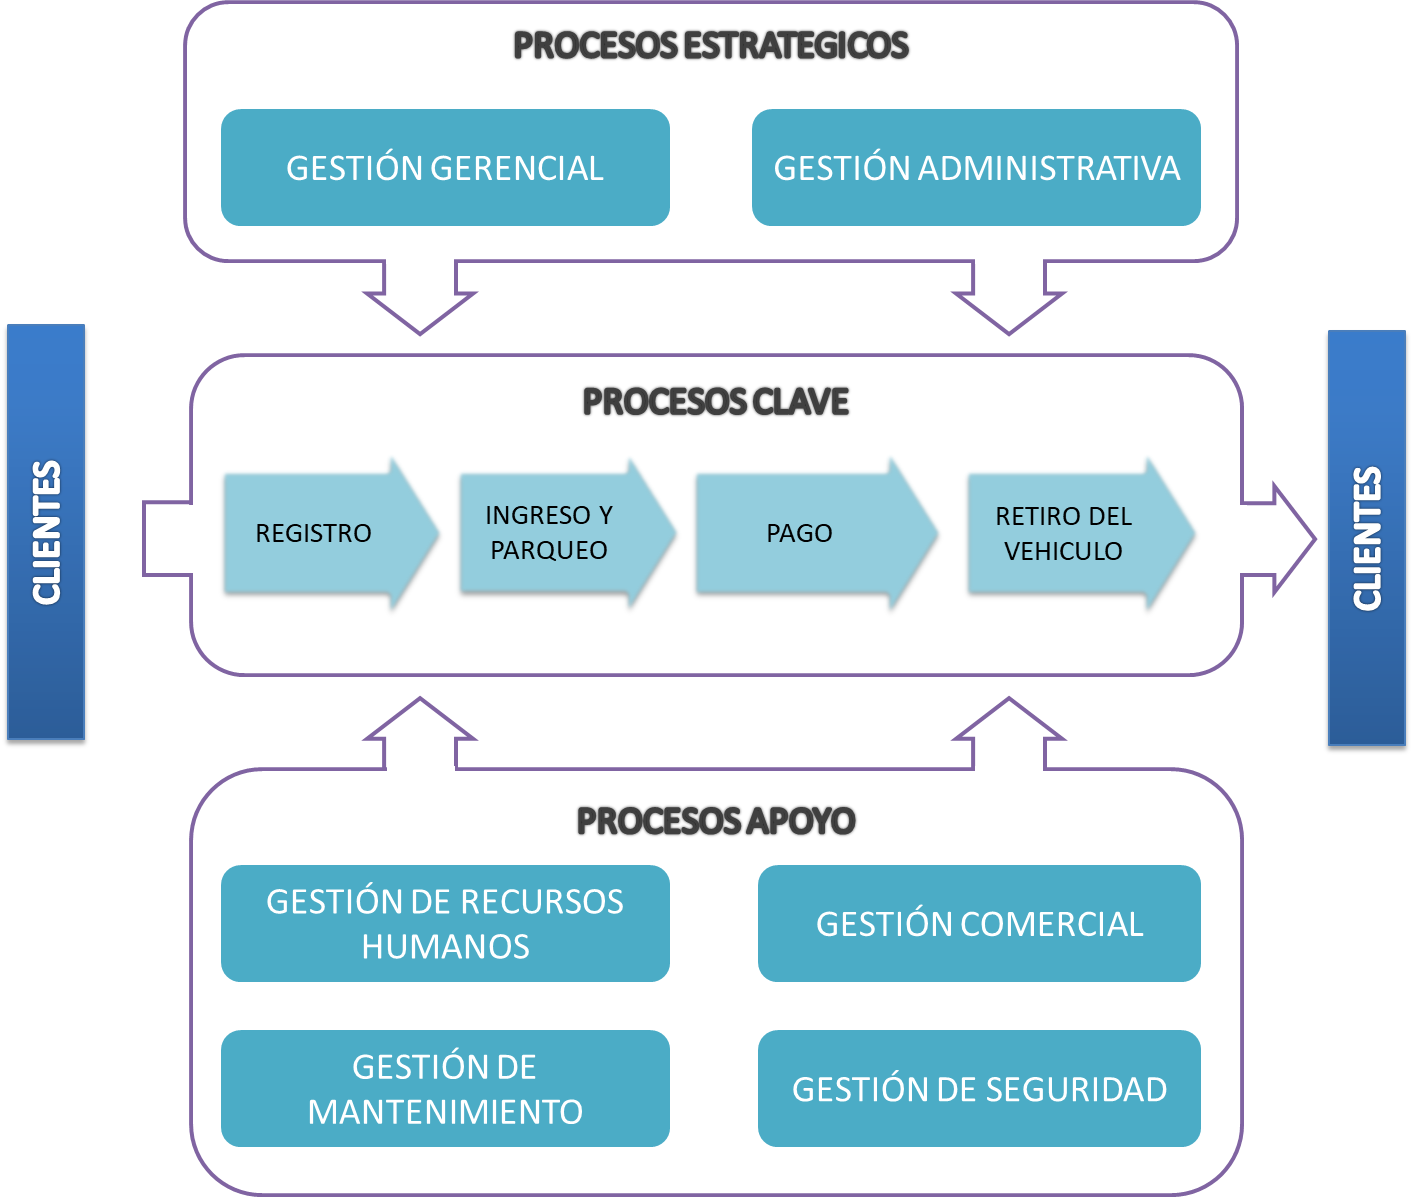
\includegraphics[width=0.8\textwidth]{imagenes/mapProcTWP}
	\caption{Mapa de Procesos de Two Wheels Paking.}
	\label{fig:awesome_image}
\end{figure}

\section{Objetivos}
\subsection{Organizacionales}
\begin{itemize}
	\item Alcanzar un amplio mercado a nivel nacional convirtiéndonos en una de las empresas pioneras de soluciones en colaboración con el medio ambiente, brindando soluciones de parqueo a aquellas personas que hacen uso de un transporte ecológico, esto con el fin de fomentar el uso de dicho transporte y contribuir al desarrollo sustentable.
\end{itemize}

\subsection{Operacionales}
\begin{itemize}
	\item Brindar la mejor calidad de servicio a nuestros clientes, mediante un equipo de trabajo altamente capacitado, convirtiéndonos en una de las empresas distritales con uno de los mejores “Goodwill”.
\end{itemize}

\subsection{Misionales}
\begin{itemize}
	\item Enfocar todos nuestros procesos al uso eficiente de los insumos y recursos, esto mediante el fomento de responsabilidad social tanto al interior como al exterior de la empresa en nuestros empleados, generando así un Impacto ambiental positivo a partir de la producción de nuestros productos y servicios.
\end{itemize}

\subsection{Estratégicos}
\begin{itemize}
	\item Posicionar a la empresa y su marca Two Wheels como una franquicia respetable de parqueo, esto mediante la estandarización y normalización de nuestros procesos, estableciendonos y generando un impacto primeramente a nivel distrital y posteriormente nacional.
\end{itemize}

\section{Valores Organizacionales}
\subsection{Amabilidad:}  En Two Wheels queremos prestar un servicio de calidad al cliente, por lo cual contamos con un equipo de trabajo capacitado el cual atenderá sus inquietudes y propuestas de la mejor manera.
\subsection{Cumplimiento:}
Sabemos que el tiempo y el dinero son recursos importantes, por eso en Two Wheels nos regimos bajo estrictos estándares y políticas internas para que las actividades estipulados se lleven a cabo en los tiempos predefinidos, los que nos convierte en una empresa sólida y seria de cara a nuestros clientes.
\subsection{Seguridad:}
En Two Wheels nos comprometemos con nuestros usuarios para brindar un ambiente seguro para sus vehículos mediante un control de acceso de usuarios efectivo e instalaciones que cuenten con una infraestructura adecuada para proteger a cada usuario y su vehículo.
\subsection{Respeto:}
En Two Wheels creemos que el pilar de toda organización es el respeto mutuo. Por eso, nuestro equipo está enfocado en brindar el mejor servicio a todos nuestros clientes, sin ninguna excepción.
\subsection{Honestidad:}
Como parte de nuestra misión, en Two Wheels creemos en el manejo transparente de nuestros procesos, ofreciendo a nuestros clientes un servicio en el cual puedan confiar.

